\renewcommand{\inputfile}{\version\ - Predrag edited 2009-08-18 slice.tex}
% siminos/thesis/chapters/slice.tex
% $Author$ $Date$

% Predrag                           Aug 18 2009
%       extracted from wilczak/blog/flow.tex

\PCedit{
\renewcommand{\Group}{\ensuremath{G}}         % Predrag Lie or discrete group

\section{\Reducedsp}
\label{sect:reducedStateSp}
% Predrag                           Aug 23 2009

    \PC{The general theory developed here should really be moved
        to \refsect{sec:mf}, this chapter should focus on the
        specific, \CLf\ example.}
In \refsect{sec:mf} we have discussed symmetry reduction by
the method of {\em moving frames} of Cartan\rf{CartanMF}, in
the formulation of Fels and
Olver\rf{FelsOlver98,FelsOlver99,OlverInv}. The basic idea is
intuitive and presumably old; for example, it is stated
without attribution as the problem 1. of Sect. 6.2 of Arnol'd
{\em Ordinary Differential Equations}\rf{arnold92}. Here we
first motivate the method by considering its
finite-rotations version, and then derive its differential
formulation, following \refref{rowley_reduction_2003}.
%
We shall refer to $\pS/\Group$ as {\em `\reducedsp'}.
In the literature this is alternatively called
`desymmetrized {\statesp},'
% `reduced \statesp,'
`orbit space,'
`quotient space,'
or
`image space,'
obtained by mapping equivariant dynamics to invariant dynamics
by methods such as
`moving frames,'
`\csection s,'
`\slice s,'
`Hilbert bases,'
\etc.
    \PC{Cite literature that uses each of the above}

\subsection{Method of moving frames, finite time steps}
\label{sect:MovFrame}
% Predrag                           Jul 19 2009
% Predrag                           Aug 12 2009

Split up the integration of a $\Group$-equivariant ODE into a
sequence of short time steps, each followed by a rotation
such that the next segment initial point is the {\slice}
fixed by a point $\slicep $ , a $(d\!-\!N)$-dimensional
hyperplane normal to the group rotation tangents
$\sliceTan_a$ at point $\slicep $:
    \PC{give formal definition of slice}
\beq
(\sspRed - \slicep ) \cdot \sliceTan_a =0
    \,,\qquad
\sliceTan_a  = \Lg_a \, \slicep
\,.
\ee{PCsectQ}
In other words, \slice\ is a Poincar\'e section for group
orbits. It is locally isomorphic to $\pS/\Group$. For any
$\sspRed \in \bar{\pS}$, $\sspRed = \LieEl(\theta)\, \ssp$ is
defined to be the rotation of $\ssp$ that lies in the \slice.
In the formulation of Fels and Olver
%\rf{FelsOlver98,FelsOlver99,OlverInv}
such a map from a \statesp\ point $\ssp$ to the group action
$\LieEl(\theta)$ is called a \emph{moving frame}.
    \PC{give a formal definition of `slice' and `coordinate
    slice.'
    }

A generic point $\slicep $ not in an invariant subspace (on
the \CLe\ $z$ axis, for example) should suffice to fix a good
\slice.
% for example a point on an \reqv\ group orbit,
% $\slicep  = \ssp_{\REQB{}1}$.
As $\slicep  \cdot \sliceTan_a =0$ by the antisymmetry of
$\Lg_a$, the slice condition \refeq{PCsectQ} determines
$\theta$ for a given $\ssp$ by
\beq
0 = \sspRed \cdot \Lg_a \, \slicep
  %= \LieEl(\theta) \cdot \hat{\ssp}   \cdot \Lg \cdot \slicep
	=\ssp \cdot \LieEl(\theta)^T \Lg_a \, \slicep
\,.
\ee{PCsectQ1}
Each
circle intersects the section exactly twice,  with the
two solutions separated by $\pi$. We select the one with a
smaller clockwise rotation angle into the \slice. The
invariant subspaces are always within the \slice, as $\Lg_a
 \ssp =0$ for $\ssp$ in an invariant subspace.
 %, so this is a nice, globally transverse \slice.

%%%%%%%%%%%%%%%%%%%%%%%%%%%%%%%%%%%%%%%%%%%%%%%%%%
% computed by PCunrot.nb
\SFIG{PCunrot}
{}{
Method of moving frames, finite time steps version,
for a 5\dmn\ flow, $\SOn{2}$ equivariant under \refeq{ZMgen}
with $x^{*}=(0,1,0,0,z)$,
$\sspRed_1=0,\;\sspRed_2>0$, \slice. A
trajectory started on the \slice, with $\sspRed_1^{(0)}
=0$, evolves for a finite time to a \statesp\ point with a
non-zero $\ssp_1^{(1)}$. Compute
the polar angle $\theta_1$ of $\ssp^{(1)}_1$ in the
$(\ssp_1,\ssp_2)$ plane. The {\em entire} \statesp\ is then
rotated (hence `moving frame') clockwise by $\theta_1$,
$\sspRed^{(1)} = \LieEl(\theta_1)\,\ssp^{(1)}$,
so that the equivalent point
on the circle lies on the \slice, $\sspRed_1^{(1)} =0$.
Thus after every finite time step followed by a rotation the
trajectory returns to the 4$\dmn$ $\sspRed_1 =0$
\reducedsp.
}
{fig:PCunrot}
%%%%%%%%%%%%%%%%%%%%%%%%%%%%%%%%%%%%%%%%%%%%%%%%%%



    \PC{generate quality PCunrot.eps from PCunrot.nb. Maybe draw
    two figures in \refFig{fig:PCunrot}, before and after the rotation.}
\refFig{fig:PCunrot} illustrates the method of moving frames,
finite time version, for an $\SOn{2}$ \slice\ motivated by the polar
form of the \CLe\ of \refsect{sect:coordChange}.
    \PC{complete \refFig{fig:PCunrot}
        - need to draw a longer segment of the initial trajectory,
        to make it clearer that the whole segment is rotated.
        $\hat{\ssp} \to \sspRed$
       }

\subsection{\Slice\ dynamics, differential formulation}
\label{sect:MovFrameODE}

% Predrag, Vaggelis                         Aug 13 2009
%           fixed the details as suggested
% Vaggelis                                  Aug 12 2009
%           \refeq{EqMotionMovFramePC} is correct
%           there are problems with the derivation.


\begin{bartlett}
I made a wrong mistake.
\bauthor{Yogi Berra}
\end{bartlett}

\noindent
By equivariance one can always write the full \statesp\
trajectory as $\ssp(t)= \LieEl(t)\,\sspRed(t)$, where the
$(d\!-\!N)$-dimensional \reducedsp\ trajectory $\sspRed(t)$
is to be fixed by some condition, and $\LieEl(t)$ is then the
corresponding curve on the $N$-dimensional group manifold of
the group action that rotates $\sspRed$ into $\ssp$ at time
$t$. The time derivative is then $\dot{\ssp}=
\vel(\LieEl\sspRed) = \dot{\LieEl}\sspRed + \LieEl\velRed$,
where the \reducedsp\ flow field is
$\velRed={d\sspRed}/{dt}$. This leads to
\[
\velRed(\sspRed) = \vel(\sspRed) - \LieEl^{-1} \dot{\LieEl} \, \sspRed
\,,
\]
where we have used the equivariance condition
\refeq{eq:FiniteRot}. The Lie group factor
\[
\LieEl^{-1} \dot{\LieEl} =
\LieEl^{-1}\frac{d~}{dt} e^{\gSpace \cdot \Lg } =
\dot{\gSpace} \cdot \Lg
\]
is the tangent field evaluated at ${\LieEl} = 1$.
Hence the flow in the
$(d\!-\!N)$-dimensional \reducedsp\ is given by:
\beq
\velRed(\sspRed) = \vel(\sspRed) - \dot{\gSpace} \cdot \Lg \, \sspRed
\,,\qquad
\velRed={d\sspRed}/{dt}
\,,
\ee{reducFlow}
for any factorization of the flow of form $\ssp(t)=
\LieEl(t)\sspRed(t)$. To actually integrate these equations
we first have to define the flow factorization by imposing
conditions on $\sspRed(t)$, and then integrate phases
$\gSpace(t)$ on a given \reducedsp\ trajectory $\sspRed(t)$.
We shall demand that the \reducedsp\ is confined to a \slice\
fixed by \refeq{PCsectQ1}.

The time derivative of the fixed slice condition
\refeq{PCsectQ}
\[
\velRed \cdot \sliceTan_a =
\vel(\sspRed) \cdot \Lg_a \slicep -
\dot{\gSpace}_a (\Lg \sspRed) \cdot \Lg \slicep
= 0
\]
expresses the group phases flow
for the slice fixed by \slicep\ in terms of
\reducedsp\ quantities $\sspRed$, $\vel(\sspRed)$
\beq
\dot{\gSpace}_a = \frac{(\vel \cdot \Lg_a \slicep)}
                       {(\Lg \sspRed) \cdot \Lg \slicep }
\,.
\ee{MFdtheta}
In the pattern recognition and 'template fitting' settings
this is called the ``reconstruction equation''%
\rf{rowley_reconstruction_2000,rowley_reduction_2003}.
The \reducedsp\ flow $d\sspRed/dt = \velRed$
\beq
% \dot{\ssp} =
\velRed = \vel - \frac{(\vel \cdot \Lg_a \slicep )}
                         { (\Lg \sspRed) \cdot \Lg \slicep }
                 \, \Lg_a \sspRed
\,.
\ee{EqMotionMovFramePC}
The equivalence classes $\Group \, \ssp = \{  \LieEl \, \ssp
| \LieEl \in \Group \}$ are manifolds called the group
orbits. We have thus replaced the dynamical system
$\{\pS,f\}$ by a reduced system $\{\bar{\pS},\bar{f}\}$ where
each  group orbit is a point in the \reducedsp\
$\bar{\pS}=\pS/\Group$. By construction $\velRed \cdot \Lg
\slicep = 0$, and  the motion stays in the
$(d\!-\!N)$-dimensional \slice.

\begin{example}% slice for \CLf
Here we can use the fact that
$- \ssp \cdot \Lg\cdot\Lg \cdot \slicep
 = (\ssp \cdot \slicep )_4 =
    x_1 x_1^{*}
   +x_2 x_2^{*}
   +y_1 y_1^{*}
   +y_2 y_2^{*}
$
is the dot-product restricted to the 4-dimensional
representation of $\SOn{2}$.

A generic  $ \slicep $ can be brought to form $ \slicep  =
(0,1,y_1^{*},y_2^{*})$ by a rotation and rescaling. Then $\Lg
\cdot \slicep   = (1,0,y_2^{*},-y_1^{*})$, and
\beq
\frac{(\vel \cdot \Lg \cdot \slicep )}{(\ssp \cdot\slicep )_4} =
\frac{\vel_1 + \vel_3 y^{*}_2 -\vel_4 y^{*}_1}
     {x_2 + y_1 y^{*}_1 + y_2 y^{*}_2}
%\frac{\vel_1 x^{*}_2 -\vel_2 x^{*}_1 + \vel_3 y^{*}_2 -\vel_4 y^{*}_1}
%     {\vel_1 x^{*}_1 + \vel_2 x^{*}_2 + \vel_3 y^{*}_1 + \vel_4 y^{*}_2}
\,.
\label{PCsectSin}
\eeq

%
%%%%%%%%%%%%%%%%%%%%%%%%%%%%%%%%%%%%%%%%%%%%%%%%%%%%%%%%%%%%%%%%%%
% CLEpcSect.png computed by  CLEfinal.nb (repo: vaggelis)
% CLEpcSect2.png computed by CLEfinal.nb (repo: vaggelis)
\begin{figure}[ht]
\begin{center}
(a) 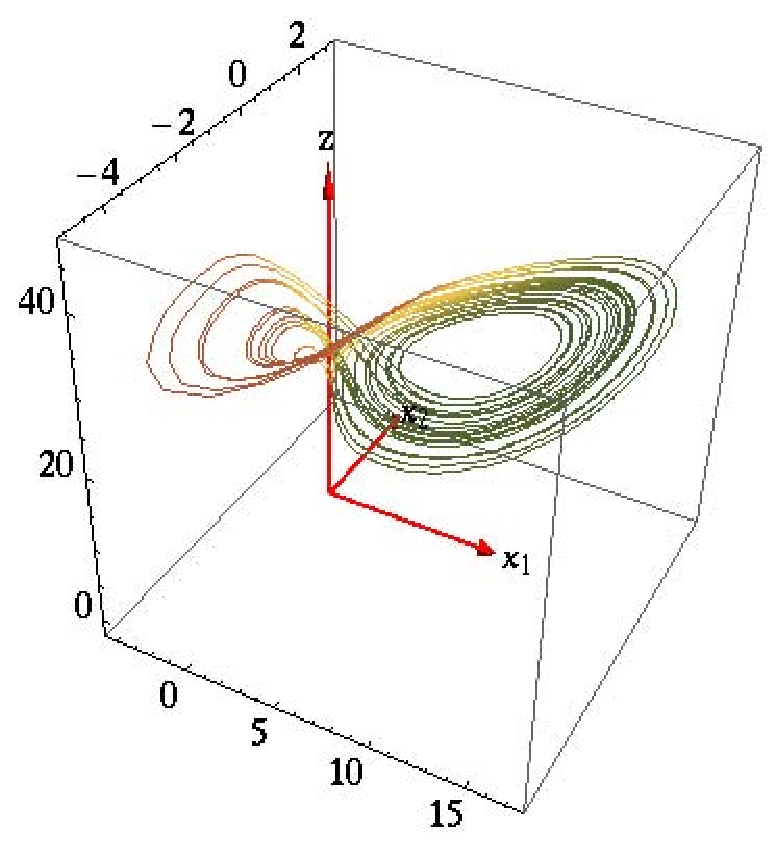
\includegraphics[width=0.40\textwidth]{../figs/CLEpcSect}
(b) 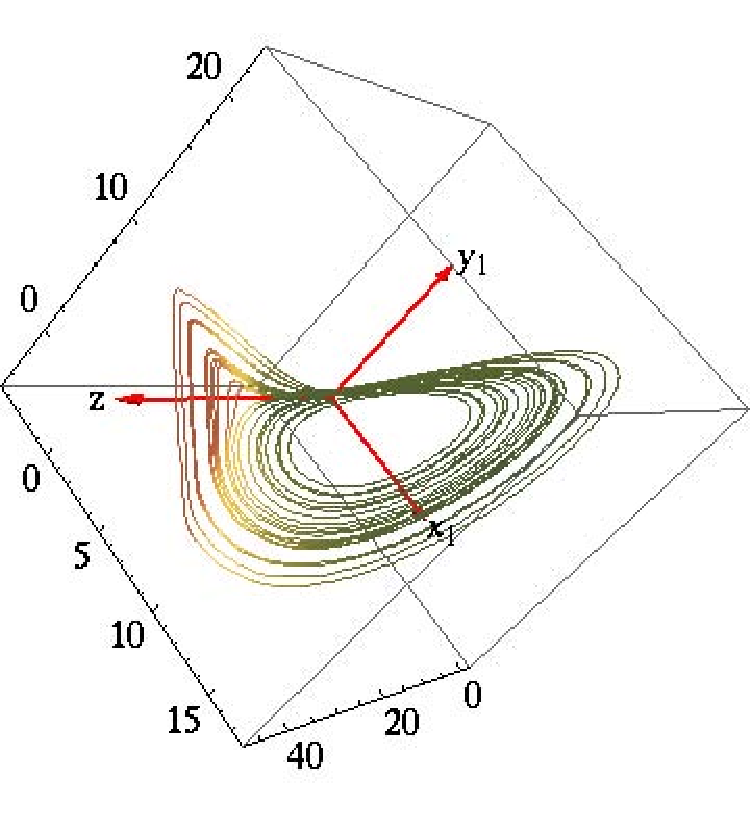
\includegraphics[width=0.43\textwidth]{../figs/CLEpcSect2}
\end{center}
\caption{
Method of moving frames, \slice\ fixed by a point on the
\reqv\ group orbit, $\slicep  = \ssp_{\REQB{}1}$. The strange
attractor of \reffig{fig:CLE} in the \reducedsp\
of \refeq{EqMotionMovFramePC}:
(a) $\{x_1,x_2,z\}$ projection,
(b) $\{x_1,y_1,z\}$ projection.
Color-coding indicates $(\hat{\ssp} \cdot \hat{\slicep })_4$
where $\hat{.}$ stands for unit vector, with green indicating values
of the inner product close to $1$ and brown indicating values
close to $0$.
    }
\label{fig:CLEpcSect}
\end{figure}
%%%%%%%%%%%%%%%%%%%%%%%%%%%%%%%%%%%%%%%%%%%%%%%%%%%%%%%%%%%%%%%%
%
    \PC{will need quality CLEpcSect.eps, CLEpcSect2.eps}
A long time trajectory of \refeq{EqMotionMovFramePC} with
$x^*$ on the \reqv\ \REQB{1} group orbit is shown in
\reffig{fig:CLEpcSect}.
\ES{I will add a scale in \reffig{fig:CLEpcSect} but it is too
late here to do it tonight.}
As initial condition
we chose an initial point on the unstable manifold
of \REQB{1}, rotated back to the \slice\ by angle $\theta$ as
prescribed by \refeq{PCsectQ1}. In \reffig{fig:CLEpcSect} we
show the part of the trajectory for $t\in\left[70,100\right]$.
The \reqv, now an equilibrium of the
\reducedsp\ dynamics, organizes the flow into a R\"ossler type
attractor. There appears to be no singularity in this
attractor although we can run into trouble with
\refeq{EqMotionMovFramePC} wherever the denominator in
\refeq{MFdtheta} vanishes, \ie, the direction of group
action on the point $\ssp$ is perpendicular to the direction
of group action on $\ssp^*$.
\ES{dropped but we need to discuss:
Apparent lack of singularities in \reffig{fig:CLEpcSect} appears
fortuitous or perhaps even a programming error.
This is a 4\dmn\ subspace, and indeed our simulations encounter
this subspace very quickly, with \reducedsp\ velocity going off to infinity.
For example, for
$\ssp^* \approx  \ssp_{\REQB{}1} = (8.48,0.077,8.48,0,26.99)$
on \reqv\ \REQB{1} group orbit,
and initial point
$\ssp(0) \approx  (4.81,0.154,7.59,0.281,15.9)$
      taken from a long run on the strange attractor, the denominator
$(\ssp(t) \cdot\slicep )_4$ vanishes at $t \approx 1.217\cdots$.
    } %end ES
%    \ES{Could this happen for the present group action and
%    choice of \slice? {\bf PC:} seems yes...}
    \PC{ in \reffig{fig:CLEpcSect}:\\
        * Mark $\ssp_{\REQB{}1}$ \\
        * Draw stable eigenvector of $\ssp_{\REQB{}1}$\\
        * State value of $\ssp_{\REQB{}1}$ somewhere
        }

%%%%%%%%%%%%%%%%%%%%%%%%%%%%%%%%%%%%%%%%%%%%%%%%%%
% computed by PCunrot.nb
\SFIG{PCunrot1}
{}{
Method of moving frames, continuous time version, for the
polar coordinates motivated $x^{*}=(0,1,0,0)$,
$x_1=0,\;x_2>0$, \slice. The \CLf\ strange attractor of
\reffig{fig:CLE} exhibits a discontinuity at
$x_2=0$ in the \reducedsp:
$\{x_2,y_2,z\}$ projection.
}
{fig:PCunrot1}
%%%%%%%%%%%%%%%%%%%%%%%%%%%%%%%%%%%%%%%%%%%%%%%%%%

Indeed, the method does encounter singularities in
subsets of \statesp.
For example, the \reducedsp\ equations \refeq{PCsectSin}
for the polar coordinates inspired \slice\
$x^{*}=(0,1,0,0)$, $x_1=0,\;x_2>0$,
%this is illustrated by \reffig{fig:PCunrot}.
%$(\rho_1,\theta_1)$ are polar coordinates, $\rho_1 =
%\sqrt{\ssp_1^{ 2} + \ssp_2^{2}}$, see \refeq{eq:CartToPol},
are given by
\beq
\dot{\ssp} = \vel - \frac{\vel_1}{\ssp_2} \Lg \cdot \ssp
\,.
\ee{EqMotionMovFrame}
A typical trajectory is shown in \reffig{fig:PCunrot}.
   \PC{this is not \reffig{fig:PCunrot} - copy correct fig
       from wilczak/blog
       }
The problem with defining the \slice\ by
\refeq{EqMotionMovFrame} is apparently that it fixes rotations
in the $(\ssp_1,\ssp_2)$ plane, not the full 4\dmn\ space.
\end{example}

\PublicPrivate{}{
\subsection{Flotsam}

The moving frames method allows the determination of (non-polynomial)
invariants of the group action by a simple and efficient
algorithm that works well in high-dimensional \statesp s.
    \PC{Vaggelis, add references here? {\bf ES}: mmm... SiminosThesis?}
    \PC{Vaggelis, why ``(non-polynomial)'' invariants?
        length$^2$ is polynomial {\bf ES}: It is the only one though.
        {\bf PC}: is this an answer?}

We decompose $\vel(x)$
in \refeq{eq:difeq} in a part $\vel_\shortparallel$ parallel
to the group action and a part $\vel_\perp$ transverse to it,
\beq
	\vel(\ssp)=\vel_\shortparallel(\ssp)+\vel_\perp(\ssp)\,,
\ee{flowSplit}
using the projection operator
\beq
 	\PperpOp_{ij}(\ssp)=\delta_{ij}-
    \frac{(\Lg \ssp)_i (\Lg \ssp)_j}{(\Lg \ssp)^2}
\ee{transvProj}
that projects a $d$-dimensional flow $v(\ssp)$ onto
flow
\beq
	\dot{\ssp}_\perp = \vel_\perp(\ssp) = \vel(\ssp)
    - \Lg \ssp \frac{(\Lg\ssp)\cdot \vel(\ssp)}{(\Lg \ssp)^2}
\ee{transvFlowSlice}
in a $(d\!-\!1)$-dimensional {\csection} transverse to the
direction fixed by the point $\ssp$.
By ignoring
the flow component that can be compensated for by an
$\SOn{2}$ rotation we quotient the flow by $\SOn{2}$.

Note, however, that a choice of
$\ssp_0$ fixes only a direction, so the reduced flow is still
equivariant under the action of discrete cyclic group $\Ztwo
= \{e,D(\pi)\}$ on $\ssp$, $\vel(\ssp)$ and the reference
point $\ssp_0$, just as was the case \refeq{LorenzR} for the
Lorenz flow \refeq{Lorenz}.
    \PC{\emph{Mea culpa}: Here I screwed up. I forgot that rotation
    moves $\vel$ and counter-moves $\ssp$ in $\vel(\ssp)$, \ie,
    acts by the Lie derivative \refeq{inftmInv}. I could never
    understand why we do not see a translational zero eigenvalue
    everywhere (the Lie group acts globally and commutatively
    right?), but only on \eqva, \reqva\ and \rpo s. Presumably
    the projection operator \refeq{transvProj} is OK for the
    \reqv\ calculation of \refeq{sect:StabEq},
    as the action of the group on $\ssp_{\REQB{1}}$ is trivial?
    Not sure how to rewrite the decomposition induced by
    \refeq{transvProj} correctly, in
    terms of the full Lie derivative action, and not only the $\Lg$
    action.
    }
}%end \PublicPrivate

\renewcommand{\Group}{\ensuremath{\Gamma}}    % Siminos Lie group

}%end \PCedit
